% =============================================================================
%  实习报告正文 —— 选题56：3D点云目标分割方法设计与实现
% =============================================================================

\section{综合训练目的与要求}

本次综合训练以“3D 点云目标分割方法设计与实现”为题，目的在于：

\begin{enumerate}[label=(\arabic*)]
  \item 运用面向对象程序设计思想（类的抽象与封装、模块解耦、接口设计）完成一个具有一定
        难度的图形学课题，并解决其中的实际问题；
  \item 掌握点云处理的基本流程：近邻搜索、法向量估计、表面分割，以及由粗到细的迭代细分；
  \item 训练用 OpenGL 进行三维数据可视化与人机交互的能力；
  \item 训练规范的程序设计文档撰写、单元测试设计与结果分析能力。
\end{enumerate}

具体的程序设计与报告要求，详见附录~\ref{app:task}。

\section{综合训练任务}

\subsection{题目与原始要求}
选题 56 属于“科研类”，原始要求为：(1) 需要一定的图形学和 OpenGL 代码基础；
(2) 读取 3D 点云文件并进行绘制；(3) 对原始点云模型实现\emph{由粗到细}的迭代分割
（需考虑点云表面朝向、点的位置分布、局部形状的连通性、表面片段的一致性与差异性度量）；
(4) 用不同颜色显示不同分割片段，实现对迭代分割过程各阶段的展示。

\subsection{需求分析}
将上述要求拆解为如下可实现的功能点，如\autoref{tab:req}所示。

\begin{table}[!htb]
  \centering
  \caption{功能需求分解}\label{tab:req}
  \begin{tabular}{@{}clp{7.2cm}@{}}
    \toprule
    编号 & 功能 & 说明 \\
    \midrule
    F1 & 点云读写 & 读取 \texttt{.ply}（ascii / 二进制小端）与 \texttt{.xyz} 文本；导出按片段着色的 \texttt{.ply} \\
    F2 & 近邻搜索 & 用 KD 树支持 $k$ 近邻查询，为法向量估计与区域生长提供邻域 \\
    F3 & 法向量与曲率 & 对每个点用 PCA 估计法向量（表面朝向）和曲率（局部平坦度） \\
    F4 & 区域生长分割 & 按表面朝向一致性与连通性把点云分成若干光滑片段 \\
    F5 & 由粗到细 & 逐层收紧法向夹角阈值，对每个粗片段继续细分，记录各层结果 \\
    F6 & 三维可视化 & OpenGL 绘制点云，支持旋转/缩放/平移、正侧俯三视图、点大小调节 \\
    F7 & 分色与回放 & 不同片段不同颜色；用滑块在各层间切换，回放由粗到细过程 \\
    F8 & 测试与数据 & 合成点云生成器 + 单元测试，验证各模块正确性 \\
    \bottomrule
  \end{tabular}
\end{table}

\section{开发环境与工具}

\begin{itemize}
  \item 语言标准：C++17；构建系统：CMake（$\ge$ 3.16）。
  \item 编译器：Apple Clang 14（macOS 12.7）；同样适用于 GCC/MSVC。
  \item 图形库：GLFW 3.4（窗口与输入）+ 系统 OpenGL 3.3 核心模式（渲染）
        + Dear ImGui 1.90（控制面板）。
  \item 文档：\nwafupaper{} 模板，Xe\LaTeX{} 编译。
  \item 说明：题目原文建议使用 PCL/OpenGL。考虑到课程“展示自身对算法的理解”这一目的，
        以及 PCL 在本机环境下依赖沉重，本项目\emph{不依赖 PCL}，KD 树、PCA 特征分解、
        区域生长等算法均自行实现。
\end{itemize}

\section{总体设计}

\subsection{处理流程}
系统的数据处理流程如\autoref{fig:flow}所示：从点云文件出发，依次经过近邻搜索、
法向量估计、区域生长，得到由粗到细的多层分割结果，最终送入 OpenGL 视口着色显示。

\begin{figure}[!htb]
  \centering
  \begin{tikzpicture}[
      box/.style={draw, rounded corners, minimum height=1.0cm, minimum width=2.1cm,
                   align=center, font=\small, fill=blue!5},
      >={Stealth[]}, node distance=0.55cm and 0.6cm]
    \node[box] (file) {点云文件\\\texttt{.ply/.xyz}};
    \node[box, right=of file] (kd) {KD 树\\$k$ 近邻};
    \node[box, right=of kd]   (nm) {PCA 估计\\法向量+曲率};
    \node[box, right=of nm]   (rg) {区域生长\\(单层)};
    \node[box, below=of rg]   (c2f) {由粗到细\\多层细分};
    \node[box, left=of c2f]   (color) {分段着色\\调色板};
    \node[box, left=of color] (view) {OpenGL 视口\\旋转/缩放/回放};
    \draw[->] (file)--(kd);
    \draw[->] (kd)--(nm);
    \draw[->] (nm)--(rg);
    \draw[->] (rg)--(c2f);
    \draw[->] (c2f)--(color);
    \draw[->] (color)--(view);
  \end{tikzpicture}
  \caption{系统数据处理流程}\label{fig:flow}
\end{figure}

\subsection{模块划分}
工程划分为“核心算法库 + 应用层”两部分，核心库不依赖任何图形界面，可单独编译与测试：

\begin{itemize}
  \item \textbf{核心库 \texttt{pcseg\_core}}：\texttt{Vec3}、\texttt{PointCloud}、\texttt{KdTree}、
        法向量估计、\texttt{Segmentation}、\texttt{PointCloudIO}、合成数据生成器；
  \item \textbf{命令行 \texttt{pcseg\_cli}}：无界面跑通“读云→法向量→分割→导出”；
  \item \textbf{图形界面 \texttt{pcseg\_gui}}：\texttt{Viewer} + \texttt{Camera}，基于 GLFW/OpenGL/ImGui；
  \item \textbf{测试 \texttt{pcseg\_tests}}：基于 CTest 的单元测试。
\end{itemize}

\section{详细设计说明}

\subsection{类设计}
按面向对象思想，把“数据、算法、显示”分别封装。主要类及其职责见\autoref{tab:class}，
类之间的关系如\autoref{fig:class}所示（核心库被三个应用共享，界面层依赖核心库而核心库
不反向依赖界面）。

\begin{table}[!htb]
  \centering
  \caption{主要类与职责}\label{tab:class}
  \begin{tabular}{@{}lp{9.5cm}@{}}
    \toprule
    类 / 模块 & 职责 \\
    \midrule
    \texttt{Vec3}        & 三维向量/点，封装加减、点积、叉积、模长、单位化 \\
    \texttt{PointCloud}  & 点云容器：坐标、法向量、曲率；包围盒、质心 \\
    \texttt{KdTree}      & 3D KD 树，建树与 $k$ 近邻查询 \\
    \texttt{SymEigen}    & $3\times3$ 对称矩阵 Jacobi 特征分解（供 PCA 用） \\
    \texttt{Segmentation}& 区域生长与由粗到细分割（\texttt{SegParams}/\texttt{SegResult}） \\
    \texttt{PointCloudIO}& PLY/XYZ 读取、着色 PLY 写出 \\
    \texttt{Camera}      & 轨迹球相机：旋转/缩放/平移、三视图、视图矩阵 \\
    \texttt{Viewer}      & OpenGL 渲染、ImGui 控制面板、串联整个流程 \\
    \bottomrule
  \end{tabular}
\end{table}

\begin{figure}[!htb]
  \centering
  \begin{tikzpicture}[
      cls/.style={draw, rounded corners, minimum height=0.85cm, align=center,
                  font=\small, fill=green!6},
      lib/.style={draw, rounded corners, minimum height=0.85cm, align=center,
                  font=\small, fill=orange!8},
      >={Stealth[]}, node distance=0.45cm and 0.5cm]
    \node[lib] (vec) {Vec3};
    \node[lib, right=of vec] (pc) {PointCloud};
    \node[lib, right=of pc] (kd) {KdTree};
    \node[lib, below=of pc] (seg) {Segmentation};
    \node[lib, left=of seg] (io) {PointCloudIO};
    \node[lib, right=of seg] (eig) {SymEigen};
    \node[cls, below=1.0cm of seg] (viewer) {Viewer};
    \node[cls, left=of viewer] (cam) {Camera};
    \node[cls, right=of viewer] (cli) {CLI / Tests};
    % 组合/依赖
    \draw[->] (pc)--(vec);
    \draw[->] (kd)--(pc);
    \draw[->] (seg)--(pc);
    \draw[->] (seg)--(kd);
    \draw[->] (seg)--(eig);
    \draw[->] (io)--(pc);
    \draw[->] (viewer)--(seg);
    \draw[->] (viewer)--(cam);
    \draw[->] (viewer)--(io);
    \draw[->] (cli)--(seg);
    \node[font=\footnotesize, align=center] at (eig.east) [right=1.4cm]
      {箭头表示\\“使用/依赖”};
  \end{tikzpicture}
  \caption{类之间的依赖关系（橙色为核心库，绿色为应用层）}\label{fig:class}
\end{figure}

\subsection{KD 树与 $k$ 近邻}
法向量估计和区域生长都要反复查询“离某点最近的 $k$ 个点”。若每次都遍历全部点是
$O(N^2)$，点数上万时很慢。KD 树按坐标轴轮流划分空间（$x\to y\to z$），建树时用
\texttt{nth\_element} 取中位数保证较平衡，查询时用一个大小为 $k$ 的大顶堆维护当前最近
的点，并利用“分割面距离”做剪枝，平均复杂度降到约 $O(\log N)$。

\subsection{法向量与曲率估计（PCA）}
对每个点取其 $k$ 个近邻，计算邻域质心，得到 $3\times3$ 协方差矩阵\cite{hoppe1992}
\[
  C=\frac{1}{k}\sum_{i=1}^{k}(p_i-\bar p)(p_i-\bar p)^{\mathsf T}.
\]
对 $C$ 做特征分解，设特征值 $\lambda_0\le\lambda_1\le\lambda_2$。最小特征值 $\lambda_0$
对应的特征向量即为该点法向量（邻域最“扁”的方向）；曲率定义为
\[
  \sigma=\frac{\lambda_0}{\lambda_0+\lambda_1+\lambda_2},
\]
$\sigma$ 越小表示邻域越平坦。$3\times3$ 对称矩阵的特征分解用经典的 Jacobi 旋转法自行
实现（见\autoref{lst:eigen}），不依赖外部线性代数库。

\subsection{区域生长分割}
区域生长把“表面朝向一致、且空间连通”的点聚成同一片段\cite{rabbani2006}，步骤如下：

\begin{enumerate}[label=(\arabic*)]
  \item 把所有未分配点按曲率\emph{从小到大}排序，越平坦的越先做种子；
  \item 取当前曲率最小的未分配点作为种子，开启一个新片段，做广度优先扩张；
  \item 对当前点的每个近邻：若其法向量与当前点法向量的夹角小于阈值
        $\theta$（一致性度量），则并入当前片段；
  \item 只有当该近邻自身也足够平坦（曲率 $<$ 曲率阈值）时，才把它作为新的扩张前沿——
        这样可以在棱边等高曲率处自然停下，不会越过物体边界；
  \item 重复直到队列为空，得到一个片段；回到 (2) 直到所有点处理完毕；
  \item 点数小于阈值的片段视为噪声丢弃，并把片段号压缩为连续编号。
\end{enumerate}

其中，法向夹角的判断用余弦实现：$|\,\hat n_{cur}\cdot\hat n_{nb}|>\cos\theta$ 即认为一致
（取绝对值是为了忽略法向量的正负朝向）。这一设计同时覆盖了题目要求的“表面朝向、
位置分布、局部连通性、一致性/差异性度量”四个方面。

\subsection{由粗到细的迭代分割}
单次区域生长只能得到一种粗细的划分。为实现“由粗到细”，本项目采用\emph{分层细分}：

\begin{itemize}
  \item 第 0 层：对整片点云用\emph{最大}的夹角阈值 $\theta_{\text{coarse}}$ 做区域生长，
        得到少数几个大块（粗）；
  \item 第 $L$ 层（$L\ge1$）：在上一层\emph{每一个}片段的内部，单独用更小的夹角阈值
        再做一次区域生长，把大块细分为更小的块；阈值从 $\theta_{\text{coarse}}$ 线性
        过渡到 $\theta_{\text{fine}}$。
\end{itemize}

这样得到的各层划分是\emph{逐层嵌套}的：细层一定是粗层的进一步切分。每层结果都被保存
下来，界面用滑块即可回放由粗到细的全过程。

\subsection{三维可视化与交互}
渲染基于 OpenGL 3.3 核心模式：点坐标和颜色分别放入两个 VBO，顶点着色器做 MVP 变换并
设置点的屏幕大小，片段着色器把方点裁剪成圆点。相机为轨迹球模型，记录观察目标、距离、
偏航角与俯仰角；鼠标左键拖动改变偏航/俯仰，滚轮改变距离，右键拖动平移目标，并提供正视、
侧视、俯视三个预设视角。控制面板用 Dear ImGui 实现，可实时调节 $k$、层数、粗/细夹角、
曲率阈值、最小片段点数等参数并重新分割，还可切换“分割结果/法向量/高度/纯色”四种着色。

\section{系统实现}

下面给出几处关键实现。完整代码见附录~\ref{app:tool} 与随附源码仓库。

\subsection{对称矩阵特征分解（Jacobi 法）}
\lstinputlisting[language=C++, caption={3x3 对称矩阵 Jacobi 特征分解},
  label=lst:eigen, firstline=23, lastline=104]{code/Eigen3x3.h}

\subsection{区域生长核心}
\lstinputlisting[language=C++, caption={区域生长：按曲率选种子、按法向夹角扩张},
  label=lst:rg, firstline=20, lastline=88]{code/Segmentation.cpp}

\section{调试与测试}

\subsection{单元测试}
项目自带轻量测试框架（用宏统计检查项与失败数），并接入 CTest。测试用例及结果见
\autoref{tab:test}，共 69 项检查全部通过。

\begin{table}[!htb]
  \centering
  \caption{单元测试用例}\label{tab:test}
  \begin{tabular}{@{}lp{8.5cm}c@{}}
    \toprule
    用例 & 验证内容 & 结果 \\
    \midrule
    Vec3        & 模长、点积、叉积、单位化 & 通过 \\
    KdTree      & $k$ 近邻结果与暴力遍历完全一致（20 组查询） & 通过 \\
    Normals     & 平面上的点法向量接近 $(0,0,1)$、曲率 $<0.02$ & 通过 \\
    PLY 往返    & 着色 PLY 写出后读回，坐标一致 & 通过 \\
    两平面      & 朝向不同且分离的两平面恰好分成 2 段，纯度 $>0.95$ & 通过 \\
    演示场景    & 由粗到细段数递增，最细层 $\ge 4$ 段，纯度 $>0.85$ & 通过 \\
    \bottomrule
  \end{tabular}
\end{table}

\subsection{分割结果与由粗到细可视化}
在内置演示场景（地面 + 球 + 圆柱 + 斜面，共 9000 点）上运行。\autoref{fig:coarse} 与
\autoref{fig:fine} 对比了由粗到细的效果：粗层（3 段）把斜面与地面并为一块；细层（5 段）
则把斜面单独分出。\autoref{fig:normal} 是法向量着色，可见地面法向一致（偏蓝）、球面法向
连续过渡（彩虹色），直观验证了法向量估计的正确性。

\begin{figure}[!htb]
  \centering
  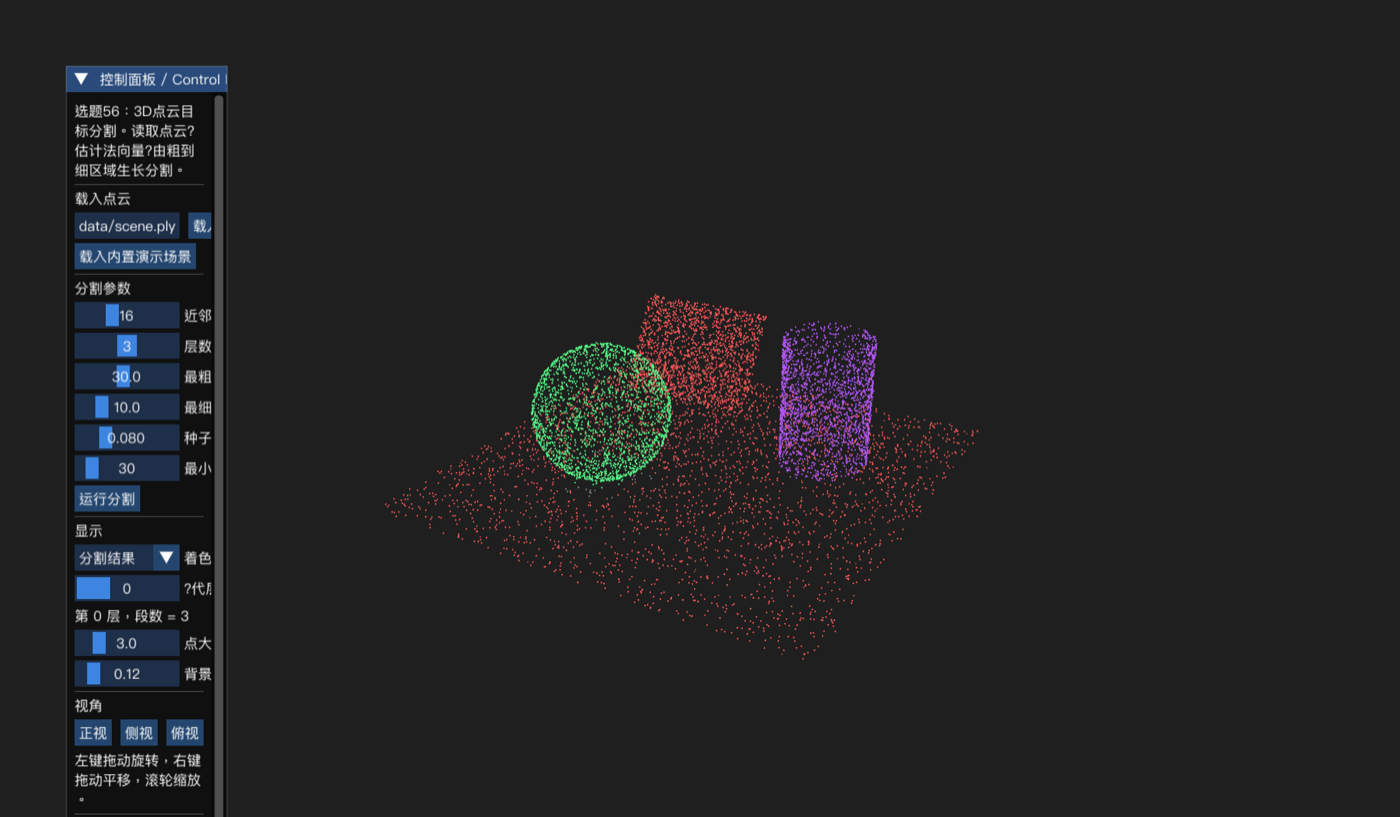
\includegraphics[width=0.86\textwidth]{figs/gui_coarse}
  \caption{粗层分割（第 0 层，3 段）：斜面与地面被合并为同一片段（红）}\label{fig:coarse}
\end{figure}

\begin{figure}[!htb]
  \centering
  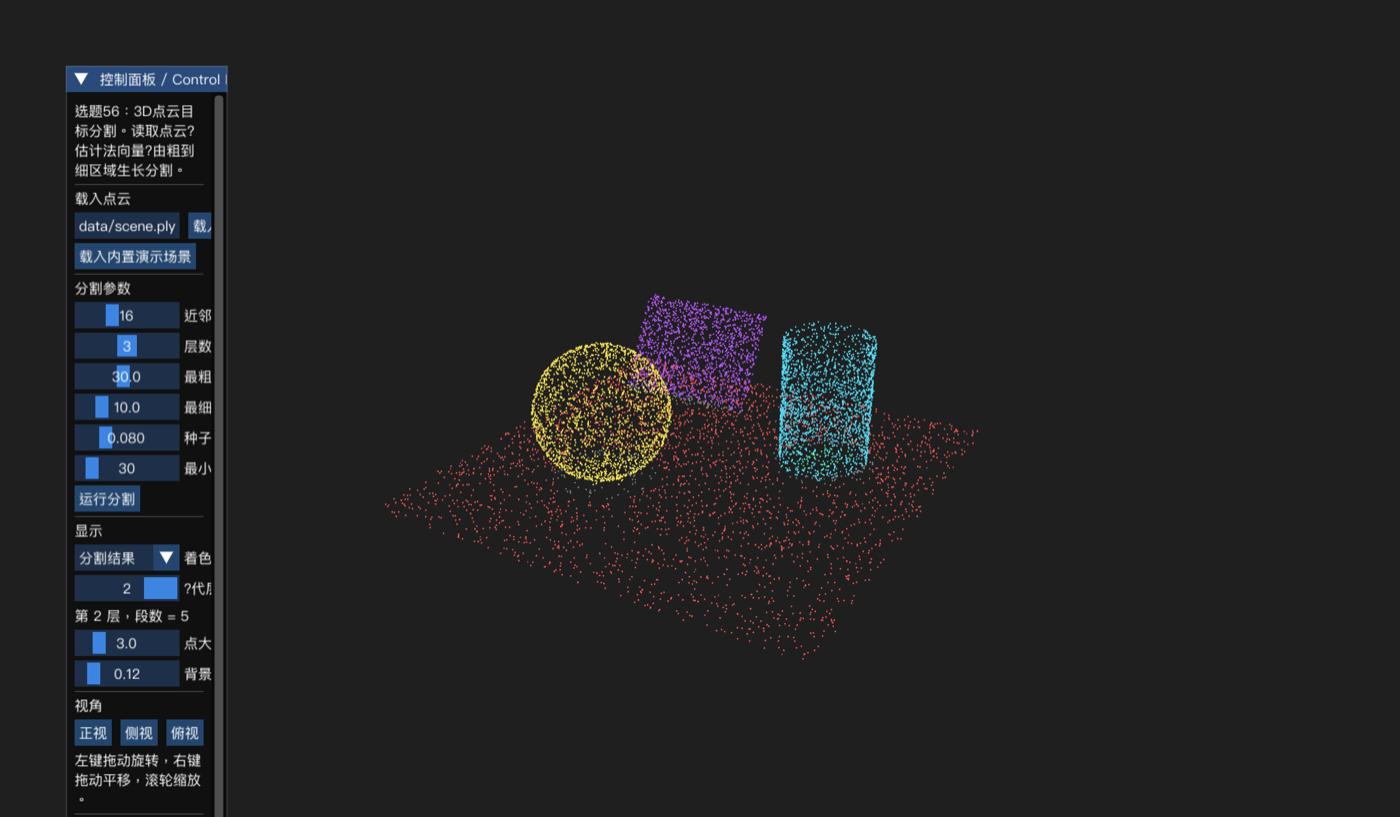
\includegraphics[width=0.86\textwidth]{figs/gui_fine}
  \caption{细层分割（第 2 层，5 段）：斜面（品红）已从地面中分离}\label{fig:fine}
\end{figure}

\begin{figure}[!htb]
  \centering
  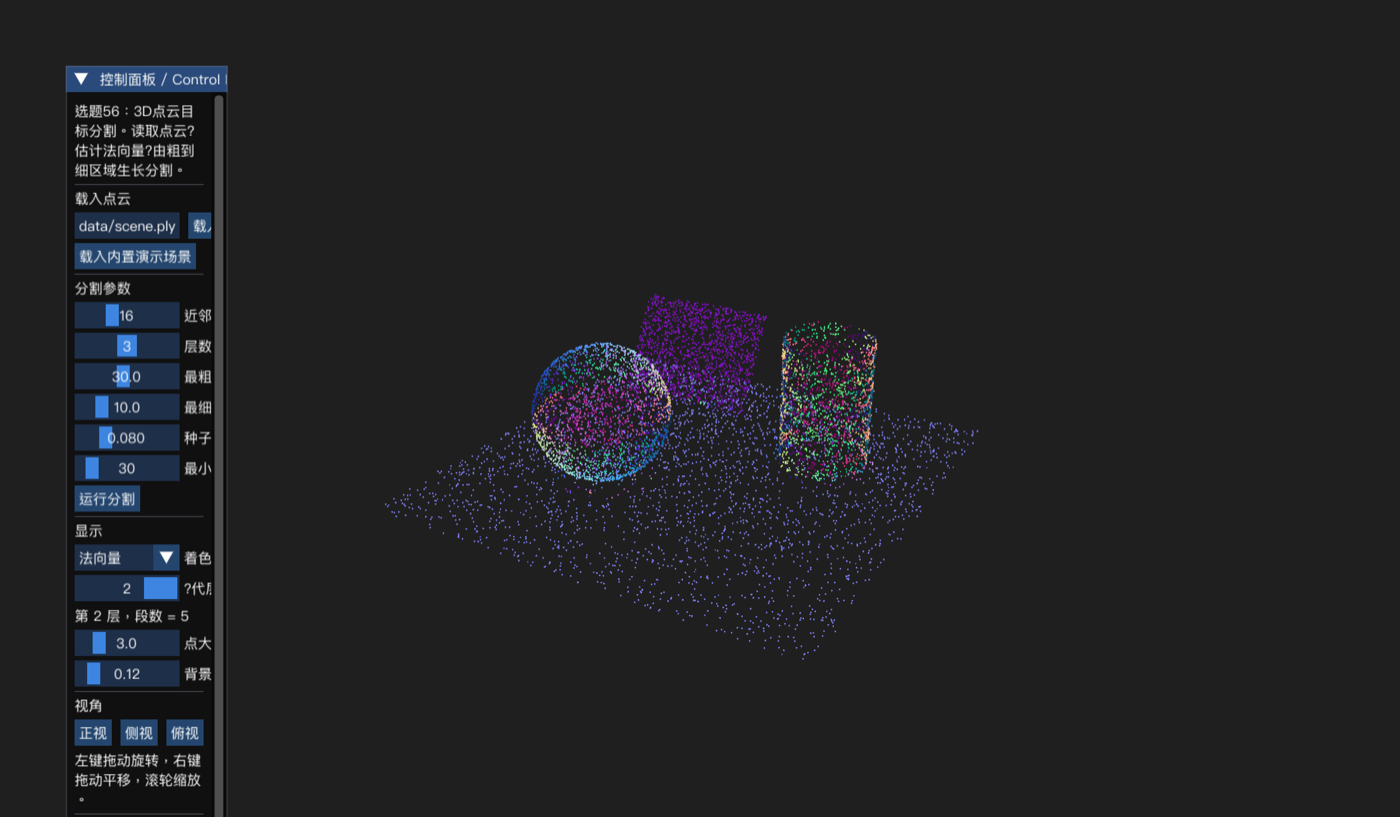
\includegraphics[width=0.86\textwidth]{figs/gui_normal}
  \caption{法向量着色：法向量 $(n_x,n_y,n_z)$ 映射为 RGB}\label{fig:normal}
\end{figure}

\subsection{性能}
在 9000 点的演示场景上，建 KD 树 + 法向量估计 + 三层分割合计约 80\,毫秒（Release 模式，
单线程），交互帧率稳定。各层段数为 $3\to3\to5$，最细层对四类目标的分割纯度约 $95.5\%$。

\subsection{已知局限}
纯区域生长在\emph{相接的锐利棱边}处可能发生“泄漏”：当两个面在棱边相连、且棱边附近法向量
呈渐变时，若中间点曲率仍低于种子阈值，区域生长会沿渐变“绕过棱角”把两个面并到一起。
在无噪声、两面恰好垂直相接的极端用例中即可复现。改进方向包括引入显式的边界/棱检测、
或在一致性度量中加入曲率突变项。本项目通过“曲率门控种子”已显著缓解该问题，并在测试中
改用\emph{空间分离}的两平面以稳定地验证分割正确性。

\section{AI 使用情况}

\begin{enumerate}[label=(\arabic*)]
  \item \textbf{使用环节}：思路梳理（区域生长与由粗到细方案的比较）、代码编写与重构、
        调试（如棱边泄漏问题的定位）、单元测试设计、实习报告与 \LaTeX{} 排版。
  \item \textbf{工具}：Claude Code（Anthropic 公司 Claude Opus 4.8 模型）。
  \item \textbf{作用}：在保证自己理解算法原理的前提下，主要用于提高编码与排版效率、
        快速定位编译/逻辑错误、对照检查测试用例的合理性。
  \item \textbf{AI 生成代码占比}：约 70\%--80\% 的初稿由 AI 协助生成，但所有算法选型、
        参数取值、测试断言和对结果的解释均经本人理解、核对与修改后确定。
  \item \textbf{遇到的问题与思考}：例如最初把“两垂直相接平面应分成 2 段”写成硬性断言，
        实际却因棱边泄漏被并成 1 段；通过分析才认识到这是区域生长的固有局限，
        进而把测试数据改为空间分离的两平面，并在报告中如实讨论。这让我体会到：
        AI 能加速实现，但对结果是否合理的判断必须由人来把关。
\end{enumerate}

\section{实习日志}

\begin{internlog}{2026/6/15}[选题与调研]
  确定选题 56（3D 点云目标分割）。调研区域生长、法向量估计、KD 树等方法，
  决定不依赖 PCL，核心算法自行实现。
\end{internlog}

\begin{internlog}{2026/6/19}[核心算法]
  完成 \texttt{Vec3}、\texttt{PointCloud}、\texttt{KdTree}、PCA 法向量、区域生长与
  由粗到细分割，并写好命令行工具与单元测试，全部测试通过。
\end{internlog}

\begin{internlog}{2026/6/24}[图形界面]
  基于 GLFW + OpenGL + ImGui 实现三维交互界面：分段着色、迭代层回放、三视图切换、
  参数实时调节，并截图用于报告。
\end{internlog}

\begin{internlog}{2026/6/26}[测试与报告]
  补充单元测试与性能分析，分析棱边泄漏局限，撰写实习报告并用 Xe\LaTeX{} 排版定稿。
\end{internlog}

\section{实习总结}

本次实践完整实现了选题 56 的全部要求：读取并绘制 3D 点云、用区域生长完成考虑表面朝向、
位置分布、连通性与一致性度量的分割、由粗到细的迭代细分、以及分色显示与各阶段回放。
在工程上，我把数据、算法与显示按面向对象思想拆成相互解耦的类与模块，核心库不依赖界面，
因此既能命令行批处理也能交互演示，并用 69 项单元测试保证了正确性。

收获主要有三点：一是真正理解了点云处理“近邻—法向—分割”的完整链条，以及 PCA 与区域
生长背后的几何含义；二是体会到面向对象的“解耦”在测试和复用上的价值——把算法与 OpenGL
分开后，算法可以脱离图形环境单独验证；三是认识到任何算法都有适用边界（如区域生长的棱边
泄漏），需要用合适的测试去暴露并诚实地分析。不足之处在于分割算法仍较基础，对噪声和复杂
真实点云的鲁棒性有限，后续可引入边界检测、超体素或基于图割的方法进一步提升效果。
